%
% LaTeX Report Assignment 3
% Ayush Jamdar EE20B018 
%


\documentclass[11pt, a4paper]{article}
\usepackage{graphicx}
\usepackage{amsmath}
\usepackage{listings}
\usepackage[]{courier}


\title{Assignment 3: Fitting Data to Models} % Title

\author{Ayush Jamdar EE20B018} % Author name

\date{\today} % Date for the report
\begin{document}		
		
\maketitle % Insert the title, author and date
\section{Aim}
%Create new section;it is autonumbered

The goal of this assignment, briefly described, is to: 
\begin{enumerate}
  \item Read data from a file and parse it.
  \item Analyse the data to extract information.
  \item Study the effect of noise on the fitting process.
  \item Plot graphs in Python.
\end{enumerate}

\section{The Assignment}

 \subsection{Introduction}
 The Python script \texttt{generate\_data.py} generates a set of data which is written out to a file named \texttt{fitting.dat}. I load the file and extract the 10 columns of this data for further operations.
 \begin{verbatim}
  time = np.loadtxt(fname='fitting.dat', usecols=0)
  data = np.loadtxt(fname='fitting.dat', usecols=(range(1, 10)))
 \end{verbatim}
  
  \subsection{Question 2: Extracting data}
  The data is a matrix with 10 columns and 101 rows. The \texttt{usecols} parameter of \texttt{loadtxt} gives the required columns. The first column is time stored in the Python variable \texttt{time}. Other nine columns are stored in \texttt{data}. The 101 rows correspond to times $0.0$ to $10.0$. What the data columns are, will be clear in the following sections.
  
  \subsection{Question 3: Noise} 
  The data columns correspond to the function 
  $$f(t)=1.05J_{2}(t)-0.105t+n(t) $$
  with different amounts of noise added. The noise is given to be normally distributed, i.e., its probability distribution is given by
$$Pr(n(t)|\sigma)=\frac{\exp(\frac{-n(t)^2}{2\sigma ^2})}{\sigma \sqrt[•]{2\pi}}$$
with $\sigma$ given by \texttt{sigma=logspace(-1, -3, 9)} \\
The noise signals $n(t)$ are plotted in Figure 0. The nine $f(t)$ functions for different noise signals are plotted. Please note that my \texttt{data} is a 2D numpy array of shape 101x9. So each column represents the \texttt{True Value} combined with a different noise distribution. Accordingly, the matrix transpose \texttt{data.T} is used in the Python code wherever necessary. 
 
   \begin{figure}[!tbh]
   	\centering
   	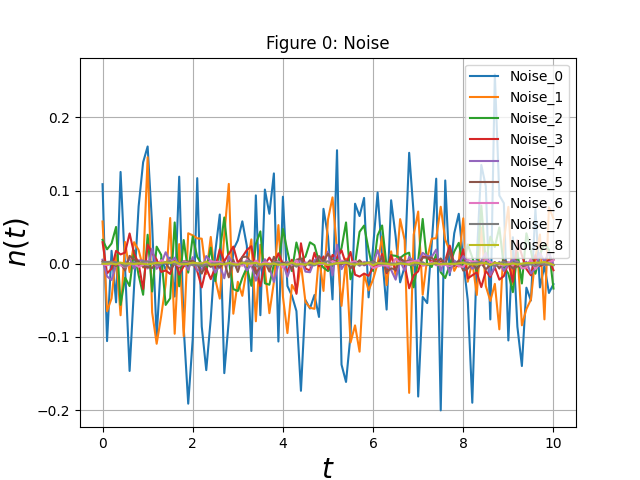
\includegraphics[scale=0.5]{Figure0_Noise.png} 

   	\label{fig:Q3}
   \end{figure} 

  \subsection{Question 4: Fitting a function to data}
  The following function is to be fitted to the data obtained:
  $$g(t, A, B)=AJ_{2}(t)+Bt$$
  I have created the following Python function \texttt{g(t, A, B)} that computes $g(t, A, B)$ for given A and B. It returns a numpy array of dimensions (101, 1) in our case.
  \begin{verbatim}	
   def g(t, a, b):
    return np.array(a * sp.jn(2, t) + (b * t))
    
   g1 = g(time, 1.05, -0.105) 
  \end{verbatim}The plot in Figure 1 shows this function \texttt{g1} fitted with all noise distributions (and the \texttt{True Value} without noise) for $A=1.05$ and $B=-0.105$.
   \begin{figure}[!tbh]
   	\centering
   	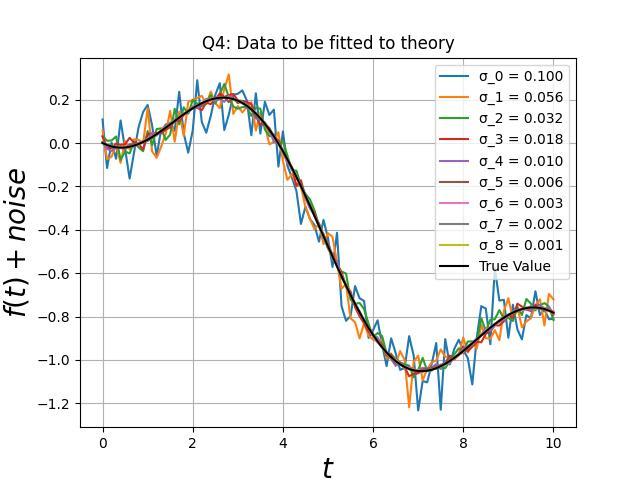
\includegraphics[scale=0.5]{Q4.jpeg} 
	\caption{Question 4}
   	\label{fig:Q4}
   \end{figure}
  
 \subsection{Question 5: Error analysis}
 Here, I have tried to analyse how much the data diverges due to noise. For the same, I have used the first column of \texttt{data}, and plotted how much every fifth data value diverges from the \texttt{True Value} by using an \texttt{errorbar} graph. The following lines do this.
 \begin{verbatim}
  plot(time, g1, 'black', label="f(t)")
  errorbar(time[::5], data.T[0][::5], sigma[0],
   fmt='ro', label='Error    bar')
 \end{verbatim}  
 The plot can be observed in Figure 2.
 \begin{figure}[!tbh]
   	\centering
   	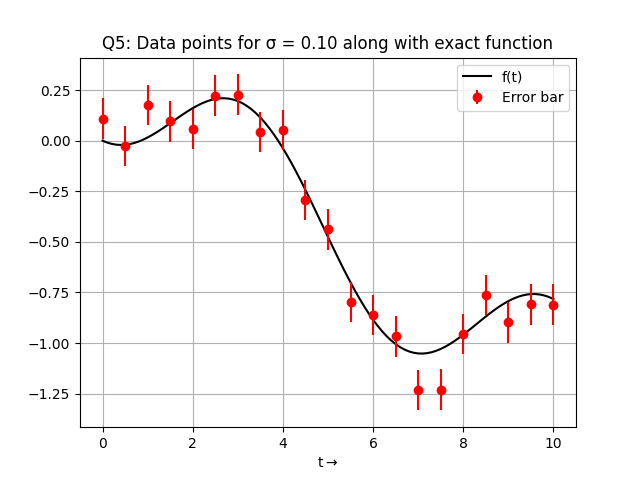
\includegraphics[scale=0.5]{Q5.png} 
	\caption{Question 5}
   	\label{fig:Q5}
 \end{figure}
 
 \subsection{Question 6: Matrix method to find \texttt{g}}
 The same function $g(t, A, B)$ obtained above for $A=1.05$ and $B=-0.105$ can also be obtained using matrix product. I have built a matrix M of dimensions (101, 2), the first column of which is the value of the Bessel function for the times in column two. The below lines of code do this.
   \begin{verbatim}
   x = np.array([sp.jn(2, time[i]) for i in range(len(time))]).T
   y = time.T
   M = c_[x, y]
   A0 = 1.05
   B0 = -0.105
   g2 = dot(M, np.array([A0, B0]).T)
   
   if g2.all() == g1.all():
    print("Part 6: Vectors are equal")
   else:
    print("Part 6: Vectors are unequal")
   \end{verbatim}
  I have compared it with the previously defined function (vector) \texttt{g1} using a special Python method \texttt{.all()}. As expected the code prints:\\ \texttt{Part 6: Vectors are equal}
  
  
  \subsection{Question 7: Mean Squared Error}
  For $A=0,0.1,\ldots,2$ and $B=-0.2,-0.19,\ldots,0$ Mean Squared Error is calculated as 
  $$\epsilon _{ij}=\frac{1}{101}\sum_{k=0}^{101}(f_{k}-g(t_{k}, A_{i}, B_{j}))^2 $$
   In Python,
  
  \begin{verbatim}
  A = arange(0, 2.1, 0.1)
  B = arange(-0.2, 0.01, 0.01)
  mean_squared_error = []
  for i in range(len(A)):
    mean_squared_error.append(zeros(len(B)))

  mean_squared_error = np.array(mean_squared_error)
  for i in range(len(A)):
    for j in range(len(B)):
        for k in range(101):
            mean_squared_error[i][j] += (data.T[0][k] - 
            g(time[k], A[i], B[j])) ** 2

  mean_squared_error /= 101
  \end{verbatim}
  Finally, $\epsilon _{ij}$ will be a numpy array of shape $(\texttt{len(A)}, \texttt{len(B)})$, where each matrix element is the mean squared error for the corresponding $A_{i}$ and $B_{j}$.
  
  \subsection{Question 8: The Contour Plot}
	As discussed in the previous section, $\epsilon_{ij}$ is a matrix with elements based on $A$ and $B$. So to understand the variation of mean squared error with $A_{i}$ and $B_{j}$, one would need a 3D plot. But thinking of it, a contour plot is also a good way to analyse because of its readability in a 2D plane. Hence, we plot the contour (See Figure 3) with the Python code:       
    \begin{verbatim}
    cs = contour(A, B, mean_squared_error)
    clabel(cs, fontsize=10)
    p = scatter(A0, B0) # to plot the exact point
    annotate("({}, {})".format(A0, B0), (A0, B0))
    \end{verbatim}
    $A=1.05$ and $B=-0.105$ are the exact values and have been marked in the plot. $\epsilon _{ij}$ has a minimum as can be understood from the plot's contour lines.
    
    \begin{figure}[!tbh]
   	\centering
   	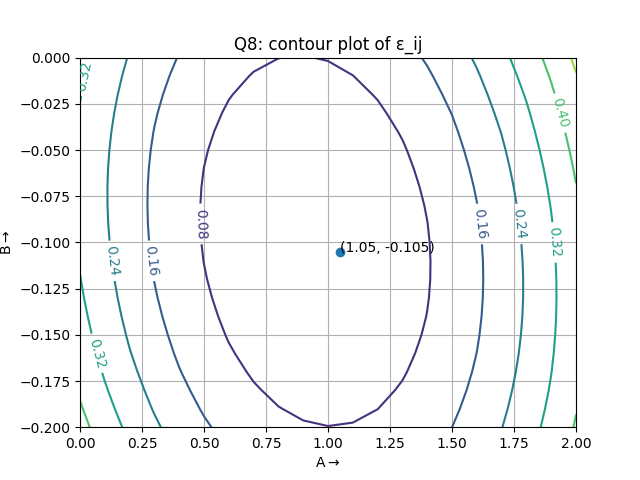
\includegraphics[scale=0.5]{Q8.png} 
	\caption{Question 8}
   	\label{fig:Q8}
   \end{figure}
    
   \subsection{Question 9 and 10: Best Estimate}
   The \texttt{lstsq} function basically solves a matrix equation $Ax=b$ by computing a vector $x$ that minimizes $|b-Ax|^2$. The equation may be under-, well-, or over-determined (i.e., the number of linearly independent rows of a can be less than, equal to, or greater than its number of linearly independent columns). If a is square and full rank, then x (but for round-off error) is the “exact” solution of the equation. If not, then x gets minimized to Euclidean 2-norm. Here, $x$ is the column $(A_{i}, B_{j})$. The code required is:

    \begin{verbatim}
		best_estimate = np.array([np.linalg.lstsq(M,
		 (data.T[i]).T)[0] for i in range(9)])
		error_in_A = A0 - best_estimate[:, 0]
		error_in_B = B0 - best_estimate[:, 1]
    \end{verbatim}

In each iteration of the list comprehension, I will get the minimized norm of A and B (The column vector of part 6) for each data column. Thus \texttt{best\_estimate} will have nine list elements $[A, B]$. Hence the columns of \texttt{best\_estimate} when subtracted from A0 and B0 will give the error (with sign; I only need magnitude for the plots) arrays. The same is plotted in Figure 4, that demonstrates variation of these errors with varying noise. The plot is quite linear for $\sigma > 0.02$, but not below it. 
    
    \begin{figure}[!tbh]
   	\centering
   	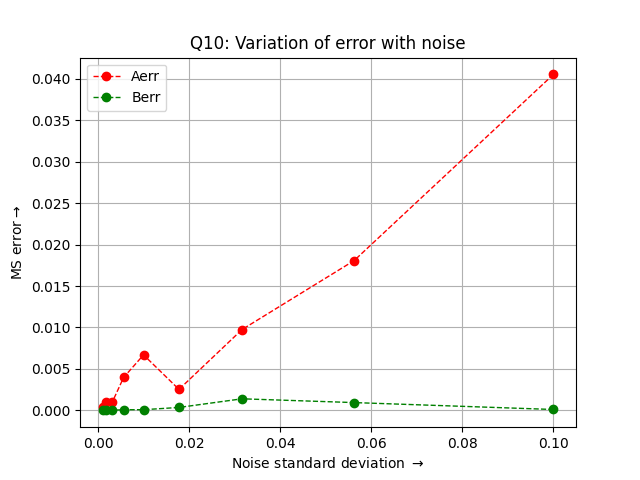
\includegraphics[scale=0.5]{Q10.png} 
	\caption{Question 10}
   	\label{fig:Q10}
    \end{figure}   
    
    \begin{figure}[!tbh]
   	\centering
   	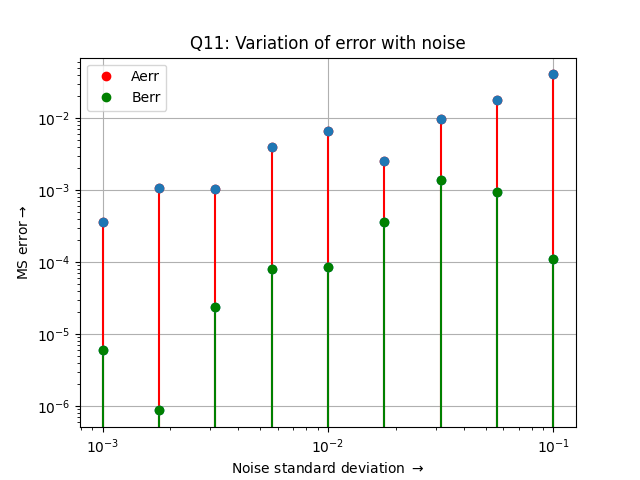
\includegraphics[scale=0.5]{Q11.png} 
	\caption{Question 11}
   	\label{fig:Q11}
    \end{figure}
    
   \subsection{Question 11: The \texttt{loglog} plot}
    The same curves of Error vs Noise Standard Deviation are here plotted on a loglog scale. See Figure 5. These can also be considered to be linear to an extent.

\section{Conclusion}
The aims that I enlisted at the beginning of this report are now seen to have been accomplished. Through every subsection, I analysed how noise and its distribution affects the main signal (function). In the later parts I studied how error is affected by $\sigma$. Through this analysis I learnt how \texttt{matplotlib} plotting functions work and how data fitting is really done. Some other inferences specific to certain subsections have been explained up there. 
    

\end{document}



 